\documentclass[11pt,a4paper]{scrartcl}
\typearea{12}
\usepackage{enumitem}
\usepackage{graphicx}
\usepackage{pstricks}
\usepackage{listings}

\usepackage{tikz}

\usepackage{pgf}
\usepackage[utf8]{inputenc}
\usetikzlibrary{arrows,automata}
\usetikzlibrary{positioning}


\tikzset{
    area/.style={
      circle,
           draw=black, very thick,
           inner sep=2pt,
           text centered,
           },
}


\tikzset{
    center/.style={
      circle,
           draw=black, very thick,
           inner sep=2pt,
           text centered,
           minimum size=2.5cm,
           },
}


\tikzset{
    neuron/.style={
      circle,
           draw=red, very thick,
           inner sep=2pt,
           text centered,
           minimum size=2.5cm,
           },
}


\tikzset{
    applic/.style={
      circle,
           draw=green, very thick,
           inner sep=2pt,
           text centered,
           minimum size=2.5cm,
           },
}



\tikzset{
    neuronfaded/.style={
      circle,
           draw=red, thin,
           inner sep=2pt,
           text centered,
           minimum size=2.5cm,
           },
}


\tikzset{
    applicfaded/.style={
      circle,
           draw=green, thin,
           inner sep=2pt,
           text centered,
           minimum size=2.5cm,
           },
}






\lstset{language=python}
\pagestyle{headings}
\markright{Computational Neuroscience - course plan}

\begin{document}
\section*{Course plan}
\begin{center}
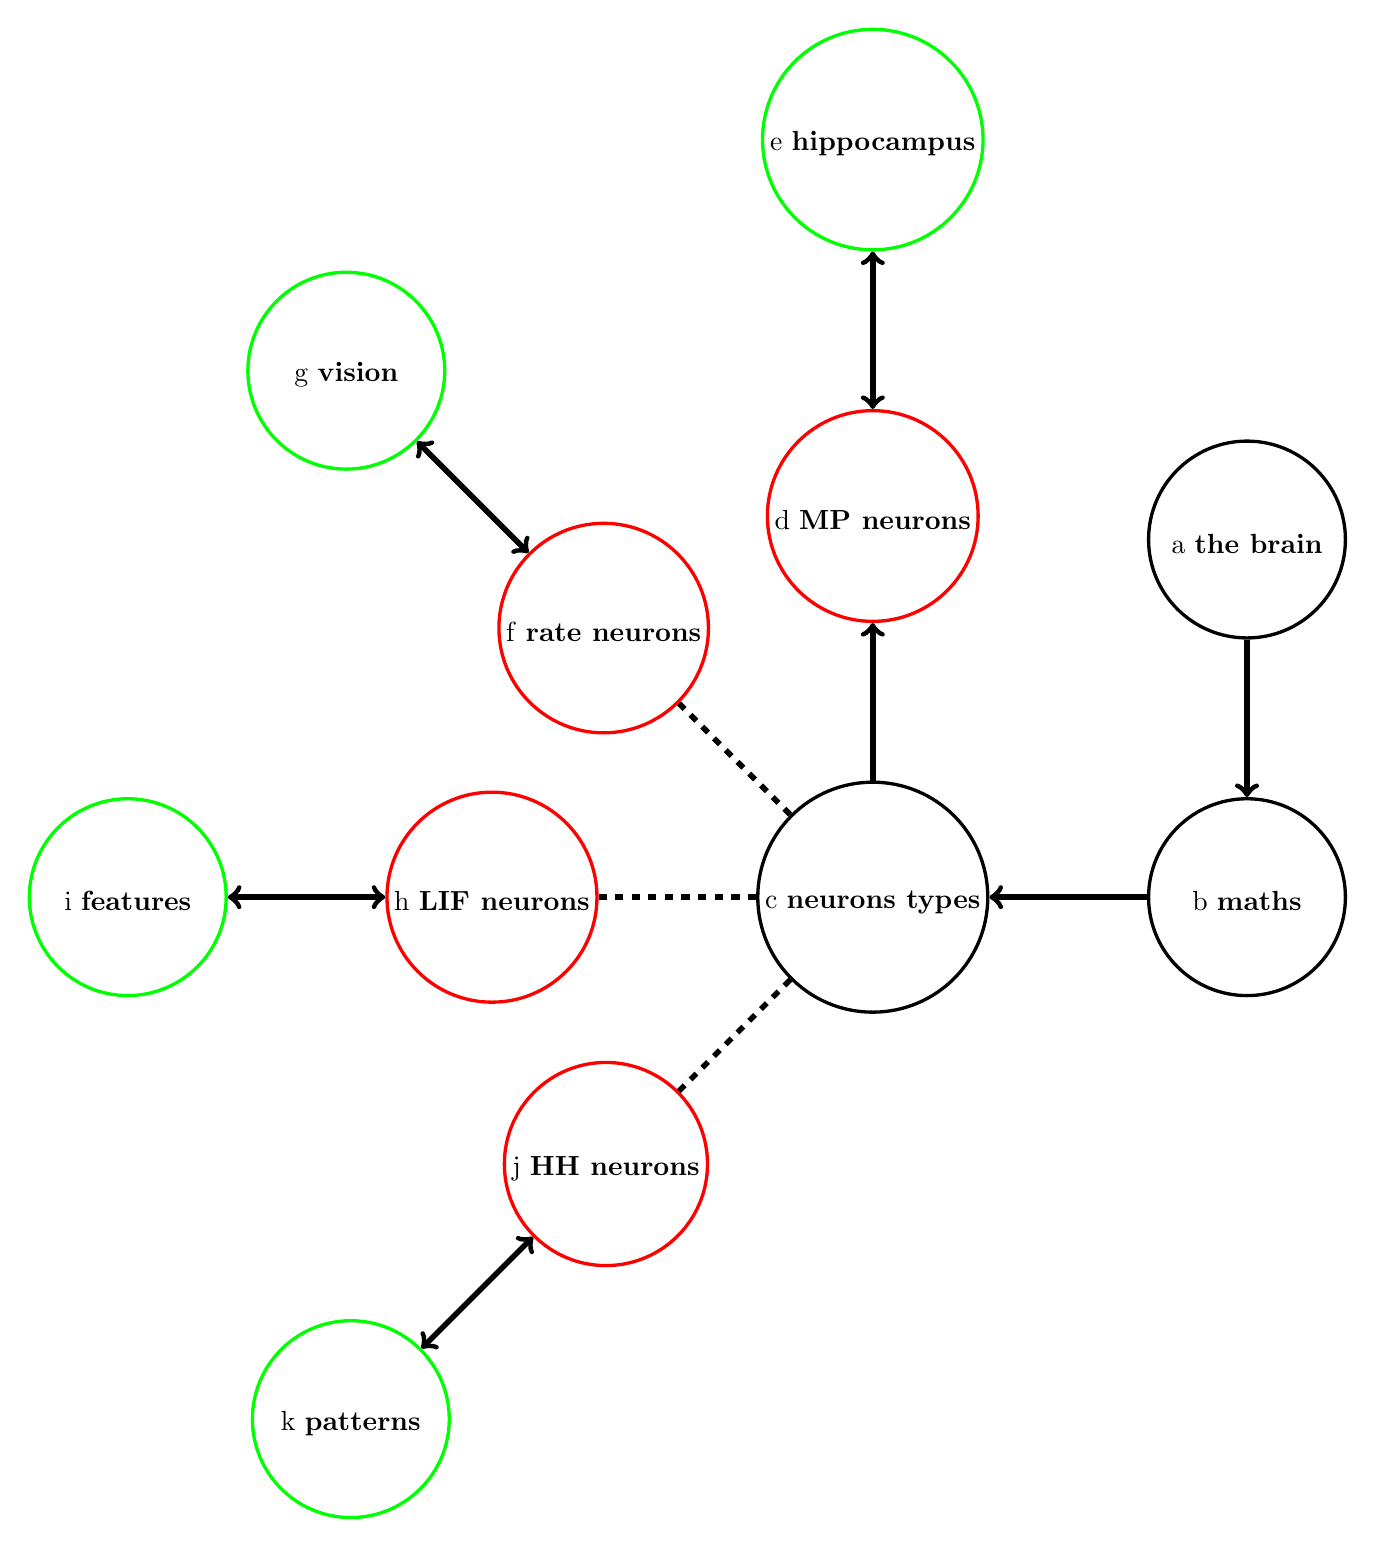
\begin{tikzpicture}

\node[center,text height=0.35cm](nt){c \textbf{neurons types}};

\node[center,text height=0.35cm,right = 2cm of nt](sc){b \textbf{maths}};
\node[center,text height=0.35cm,above = 2cm of sc](tb){a \textbf{the brain}};


\path (tb) edge[->,line width=2pt](sc);
\path (sc) edge[->,line width=2pt](nt);



\node[neuron,text height=0.35cm,above = 2cm of nt](on){d \textbf{MP neurons}};
\node[applic,text height=0.35cm,above = 2cm of on](hpc){e \textbf{hippocampus}};

\path (nt) edge[->,line width=2pt](on);
\path (on) edge[<->,line width=2pt](hpc);

\node[neuron,text height=0.35cm,above left = 2cm of nt](rn){f \textbf{rate neurons}};
\node[applic,text height=0.35cm,above left = 2cm of rn](vis){g \textbf{vision}};

\path (nt) edge[-,line width=2pt,style=dashed](rn);
\path (rn) edge[<->,line width=2pt](vis);


\node[neuron,text height=0.35cm,left = 2cm of nt](ln){h \textbf{LIF neurons}};
\node[applic,text height=0.35cm,left = 2cm of ln](pla){i \textbf{features}};

\path (nt) edge[-,line width=2pt,style=dashed](ln);
\path (ln) edge[<->,line width=2pt](pla);


\node[neuron,text height=0.35cm,below left = 2cm of nt](hn){j \textbf{HH neurons}};
\node[applic,text height=0.35cm,below left = 2cm of hn](pat){k \textbf{patterns}};

\path (nt) edge[-,line width=2pt,style=dashed](hn);
\path (hn) edge[<->,line width=2pt](pat);

% \node[neuronfaded,text height=0.35cm,below = 2cm of nt](nm){\textcolor{gray}{l \textbf{neural mass}}};
% \node[applicfaded,text height=0.35cm,below = 2cm of nm](eeg){\textcolor{gray}{m \textbf{fmri / eeg}}};

% \path (nt) edge[-,line width=1pt,draw=gray,style=dashed](nm);
% \path (nm) edge[<->,line width=1pt,draw=gray](eeg);

% \path (on) edge[->,line width=2pt](rn);
% \path (rn) edge[->,line width=2pt](ln);
% \path (ln) edge[->,line width=2pt](hn);
% \path (hn) edge[->,line width=1pt,draw=gray](nm);

\end{tikzpicture}
\end{center}

\section*{Key to the plan}


\begin{enumerate}[label=(\alph*)]
\item \textbf{the brain:} A quick and easy outline introduction to the brain and neuroscience.
\item \textbf{some math:} An introduction to differential equations and their numerical solution.
\item \textbf{neuron types:} An overview of neuronal modelling.
\item \textbf{\textcolor{red}{MP neurons:}} The McCulloch-Pitts model of neurons, simple synapses.
\item \textbf{\textcolor{green}{hippocampus:}} Description of the hippocampus and auto-associative memory computations.
\item \textbf{\textcolor{red}{rate neurons:}} The rate model of neurons, including
  receptive fields.
\item \textbf{\textcolor{green}{vision:}} The visual pathway; V1, receptive fields in V1 and sparse coding.
\item \textbf{\textcolor{red}{LIF neurons:}} Spiking, spike triggered averages and time histograms, the leaky integrate and fire neuron.
\item \textbf{\textcolor{green}{features:}} Spike timing dependent plasticity and feature extraction.
\item \textbf{\textcolor{red}{HH neurons:}} Ion channels and Hodgkin-Huxley neurons;
  Morris-Lecar and other models.
\item \textbf{\textcolor{green}{patterns:}} Some ideas from dynamical systems, central pattern generators.
% \item \textbf{\textcolor{red}{neural mass:}} Neural mass models and field equations for neurons.
% \item \textbf{\textcolor{green}{fmri / eeg:}} From neurons to the brain; modelling the interactions of brain regions.
\end{enumerate}

\section*{Rough lecture list}
This is a rough guide, it might change as the course progresses.

\begin{enumerate}

\item Introduction to the course and to the brain. (a 01-29 Conor)
\item More on the brain. (a 01-31 Conor)
\item Still more on the brain. (a 02-05 Conor)

\item Introduction to differential equations. (b 02-07 Conor)
\item Numerical solutions to differential equations. (b 02-12 Conor)

\item Modelling neurons. (c 02-14 Cian)
\item The McCulloch-Pitts neuron, Perceptrons, and Hopfield networks. (d 02-19 Cian)

\item The Hippocampus. (e 02-21 Cian)
\item Models of hippocampal computations: Pattern separation, pattern completion, and path integration. (e 02-26 Cian)

\item Firing rates, dealing with neuronal data, receptive fields. (f 02-28 Cian)
\newline \newline [Reading week]
  
\item The visual system. (g 03-12 Cian)

\item V1 and sparse coding. (g 03-14 Cian)
\item Spikes and analysing spike date. (h 03-19 Cian)

\item Simple models of neurons: leaky integrate and fire neurons. FI curves (h 03-21 Cian)
\item Synapses and synaptic plasticity. (i 03-26 Rui)
\item Long term plasticity. (i 03-28 Rui)
\item STDP and feature extraction. (i 04-02 Rui)
\item T.B.D. (04-04)
\newline \newline [Easter break, 3 weeks]
  
\item Ion channels. (j 04-30 Conor)
\item The Hodgkin-Huxley equation and spikes. (j/k 05-02 Conor)

\item Dynamical systems approachs, the Morris-Lecar model, phase diagrams. (k 05-07 Conor)
\item Central pattern generators, bursting. (k 05-09 Conor)

\end{enumerate}

\end{document}

